% Paper for CGAT
\documentclass[10pt, conference, compsocconf]{IEEEtran}

\usepackage{float}
%\usepackage{url}
\usepackage{graphicx}
\usepackage{subfig}
\usepackage{color}

\begin{document}

\title{CGAT In The Hat}

% author names and affiliations
% use a multiple column layout for up to two different
% affiliations

\author{\IEEEauthorblockN{Eriq Augustine, Ryan Hnarkis, Aldrin Montana, Ryan Verdon, Tyler Yero}
\\
\IEEEauthorblockA{Department of Computer Science\\
Cal Poly, San Luis Obispo\\
 \textsf{\{eaugusti, rhnaraki, amontana, rverdon, tyero\}@calpoly.edu}
}
}

\maketitle

\thispagestyle{empty}
\pagestyle{empty}

\section{Introduction}\label{sec:introduction}
Gene annotation is the process of associating metadata about a gene with the
contig, a dna sequence, on which the gene resides.\cite{annotation} This metadata is necessary for conducting
genomic research projects and analysis involving the contig's genomic sequence.
Currently, there is no specialty gene annotation software. Genome browsers
all maintain lots of genomic data and are used when manually annotating genes,
but do not provide a user-friendly interface. While genome browsers
will likely never be replaced (UCSC genome browser, etc. are well
established\cite{ucscbrowser, ncbi}), it would be desirable to have a software system that better
accommodates the visual and informational needs of gene annotation.

\textit{CGAT} is a web-based gene annotation application designed with
usability, simplicity, and efficiency in mind. It is not a feature-rich and data-rich
 genome browser like the \textit{UCSC genome brower}. Nor is \textit{CGAT}
designed to be a replacement for other genome browsers in any aspect other than
gene annotation. Other gene browsers attempt to accommodate many needs of the
biology community and so offer many features, and a cluttered, chaotic
interface. Gene annotation, while not a trivial task, can be well-serviced by a
simple data model. Ideally, by focusing on a simple data model, \textit{CGAT}
is able to provide a clean, streamlined experience. \textit{CGAT} aims to
provide users with a way to view gene annotations without extra, unnecessary
information obscuring their view while also embodying a Wikipedia-like emphasis
on collaboration and openness.

This paper discusses the progress that has been made this quarter and the future work that 
still needs to be done. The rest of the paper is as follows. Section \ref{sec:background} discusses
the common terms and biological meanings used in the project. Section \ref{sec:motive} discusses the
motivation for creating CGAT. Section \ref{sec:choice} explains why we chose MongoDB
as our backend. Section \ref{sec:implementation} goes into the details of how
our backend and frontend are implemented currently. Section \ref{sec:results} discusses
the results of our demo to our customer. Lastly, section \ref{sec:future} 
describes the future work still left to do.

\section{Background}\label{sec:background}

\section{Motivation}\label{sec:motive}
Dr. Anya Goodman, a professor in the Chemistry department at Cal Poly, San Luis
Obispo, offers a bioinformatics course that covers several aspects of gene
annotation. Her work is a part of the Genomics Education Partnership (GEP) at 
Washington University in St. Louis.\cite{gep} The goal of GEP is to teach undergrad students
in Biology how to annotate genes and other features in raw sequence data.
The CGAT project is spearheaded by Ryan Verdon to accommodate Dr.
Goodman's needs and ideas for ideal gene annotation software.

\section{Database Choice}\label{sec:choice}
The choice for backend database was between MySQL, Couchbase, and MongoDB.
We included MySQL in the options because its the standard that websites tend to use. Then we included both
Couchbase and MongoDB in our considerations because they are popular NoSQL database of different types of NoSQL
databases. Couchbase is a key-value store whereas MongoDB which is a document-store.

We ended up using MongoDB for several reasons. First, the document structure was extremely helpful when storing
relations. We ended up attaching a lot of data on our relations that would of been a pain to store in SQL but being
able to store the data as complex objects in JSON was super helpful. Second, being able to store the data in JSON
(BSON in MongoDB) made it extremely easy to retrieve and use the data in a web application. Because of these two reasons
we narrowed our choices down to MongoDB and Couchbase. 

When we were deciding between MongoDB and Couchbase we looked at the features they 
provided and noticed several things. First, Couchbase currently is a pure key-value store it has
no idea what the structure of the value. Unlike MongoDB, which can query for fields inside an 
object specified by a key. This feature of MongoDB makes updating relations (which we 
have a lot of) super easy. Second, Couchbase provides a huge
cluster/map reduce overhead that is not necessary for our data. Therefore we choose to use
MongoDB for the CGAT database.

\section{Implementation}\label{sec:implementation}
CGAT uses a standard LAMP (Linux Apache MySQL PHP) stack with MySQL traded out for MongoDB.

\subsection{Backend}
The \textit{backend} of the system consists of a PHP server connecting to a MongoDB database.
We do not use any templating systems.
We chose PHP for the backend because we did not require most of the functionality of a templating system, and we wanted a simple
system that can be easily understood when passed off to the next generation.

PHP and MongoDB work together very nicely and MongoDB's PHP connector is fully featured \cite{phpMongo}.

\subsubsection{Database Schema}
Although we use MongoDB which does not enforce a specific schema, by convention we enforce a schema on our documents.
MongoDB uses BSON (Binary JSON). BSON is an extended JSON format that supports additional types like a datetimes \cite{bson}.

The schemas for our four JSON objects are shown in Figures \ref{fig:JSON-contig}, \ref{fig:JSON-annotation},
\ref{fig:JSON-user}, and \ref{fig:JSON-group} in Appendix \ref{sec:data_models}.

\subsubsection{API}
CGAT is an entirely API driven product. The API is central to all the behavior.
The API supplies \textbf{all} the information that is displayed in the UI.
This is a very important design choice. Having the API be the sole data provider and manipulator for the system
means that all functionality can be programmatically provided and different applications can present the same
functionality with a different UI.

The API accepts GET and PUT requests (depending on the action) and will always return a JSON response.

The current API supports 21 different calls, 7 GET requests and 14 POST actions.

\paragraph{GET Requests}
\begin{itemize}
\item administration\_info - Provides the user with meta information information that the user would need to perform administrative tasks such as creating a group or assigning a task.
\item annotation - Provide the user with information about an specified annotation.
\item contig - Get information about a specific contig.
\item gene - Get information about a specific gene.
\item group - Get information about a specific group.
\item help - Get help information on a specific topic.
\item user\_profile - Get the profile information about a specific user. If the user is logged in and requests information about themselves, more information is provided.
\end{itemize}

\paragraph{POST Actions}
Most POST actions require that the user is logged in.

\begin{itemize}
\item assign\_task - Ask a group of people to perform an annotation.
\item cancel\_notification - Clear a notification from a user.
\item create\_annotation - Create a new annotation of a contig.
\item create\_group - Create a group.
\item join\_group - Join a group.
\item leave\_group - Leave a group.
\item login - Login.
\item logout - Logout.
\item parse\_fasta - Upload a FASTA file to the server, parse the contents, and returned the parsed structure.
\item register - Register a new user.
\item save\_annotation - Save a work-in-progress annotation.
\item set\_help - Upload a help page.
\item submit\_annotation - Submit a finalized annotation.
\item upload\_contig - Upload a contig into CGAT.
\end{itemize}

\subsection{Frontend}
CGAT's frontend uses standard web technologies (HTML, Javascript, and CSS).
CGAT uses many HTML5/CSS3 features such as transforms and pseudo-elements.

Because the entire system is API based, the frontend heavily relies on asynchronous fetches (AJAX).

\section{Results}\label{sec:results}
We demoed CGAT to Dr. Anya Goodman on the 19th of November. She was pleased with
the work accomplished so far. But she had numerous recommendations for things to fix and update.
We have taken her ideas and attempted to get as much fixed in the last weeks of the quarter.
Some of the notable fixes were removing some of the "prettiness" from the site, making
buttons look more like buttons, and changing some of the words and terminology used on the site.

\section{Future Work}\label{sec:future}
The future work that is left to be done on CGAT falls into several categories. 

\subsection{Missing use cases}
We still need to add some of the main use cases that Dr. Goodman wanted. This includes things like
user leveling and immediate feedback on annotations. 

\subsection{Bug fixes}
We know of several bugs that still need to be fixed based on feedback from the demo with
Dr. Goodman.

\subsection{New features}
New features for CGAT will most likely be desired after user feedback.

\subsection{Accessibility}
Need to test the accessibility of the site. This includes things like the color set used
and text size.


\bibliographystyle{acm}
\bibliography{refs}


\onecolumn
\appendices

\section{JSON Data Models}\label{sec:data_models}
\centering
Here are diagrams depicting our JSON data model.

\begin{figure*}[h]
   \centering
   \subfloat[Contig format]{\label{fig:JSON-contig}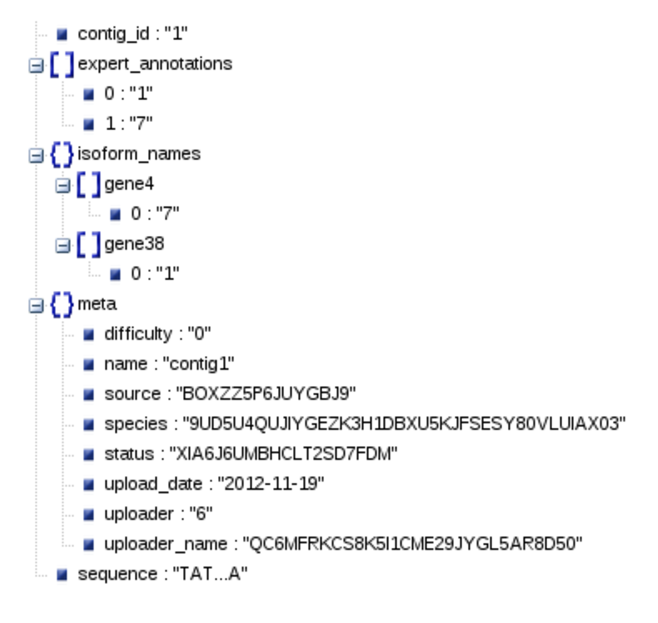
\includegraphics[height=70mm]{contig.eps}}
   \subfloat[Annotation format]{\label{fig:JSON-annotation}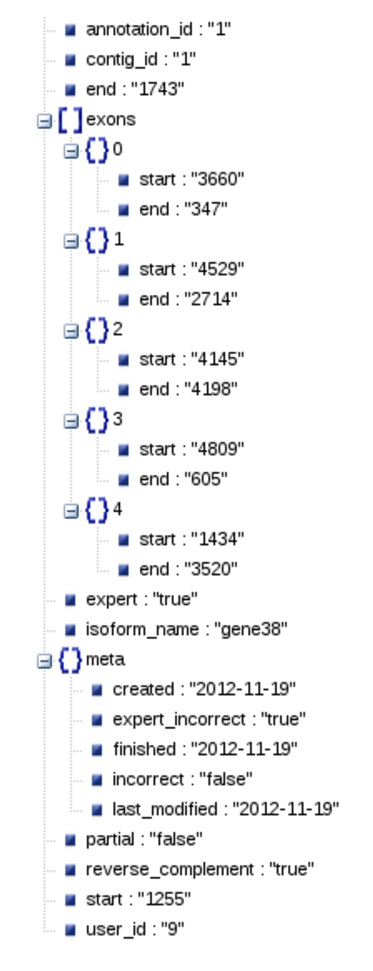
\includegraphics[height=80mm]{annotation.eps}}
   \caption{JSON format for Contigs and Annotations.}
\end{figure*}

\begin{figure*}[h]
   \centering
   \subfloat[User format]{\label{fig:JSON-user}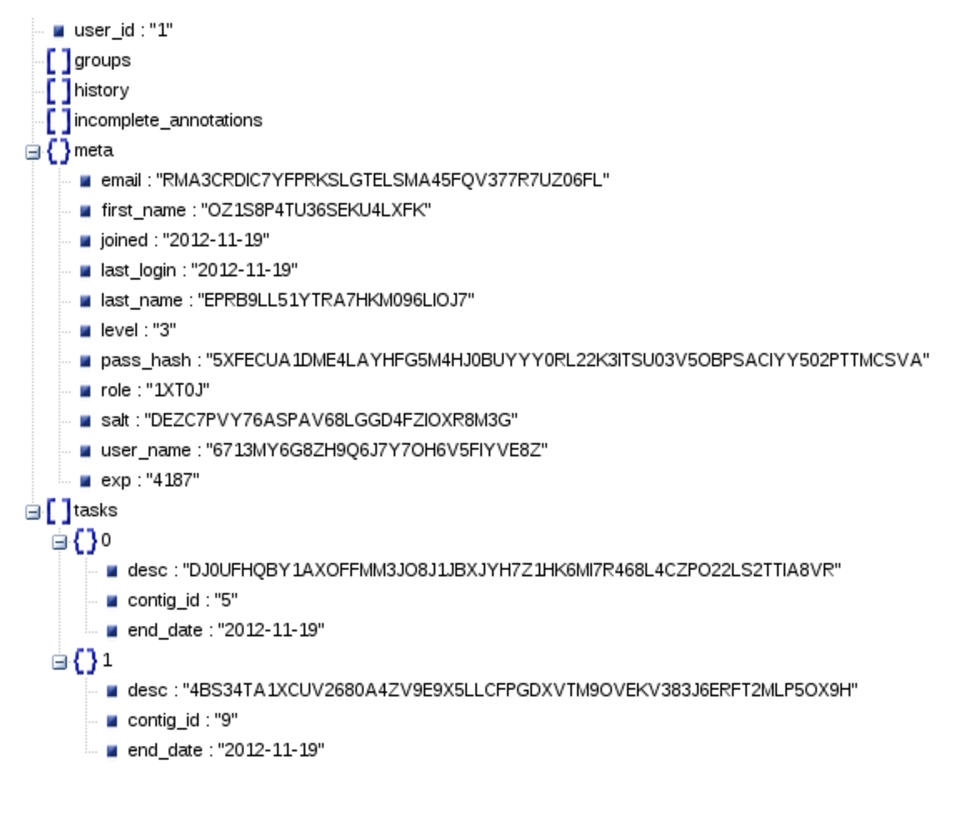
\includegraphics[height=90mm]{user.eps}}
   \subfloat[Group format]{\label{fig:JSON-group}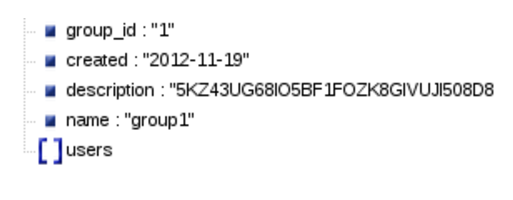
\includegraphics[height=25mm]{group.eps}}
   \caption{JSON format for Users and Groups.}
\end{figure*}


\end{document}
